\documentclass[12pt]{article}

\usepackage{bbm}
\usepackage{fancyhdr}
\usepackage{titling}
\usepackage{enumitem}
\usepackage{amsmath}
\usepackage{dsfont}
\usepackage{amsfonts}
\usepackage{amssymb}
\usepackage{amsthm}
\usepackage{geometry}
\usepackage{tikz}
\usepackage{algorithm}
\usepackage{algpseudocode}
\geometry{verbose,tmargin=1in,bmargin=1in,lmargin=1in,rmargin=1in}
\renewcommand{\vec}[1]{\mathbf{#1}}
\newcommand{\dec}{\text{dec}}
\newcommand{\divi}{\mathbin{\textnormal{div}}}
\title{Homework 1}
\author{Satvik Prasad}
\date{}
\newtheorem{lemma}{Lemma}[section]
\fancypagestyle{plain}{%
  \fancyhf{}
  \fancyhead[L]{\theauthor}
  \fancyhead[R]{\thedate}
}
\pagestyle{plain}
\makeatletter
\def\@maketitle{%
  \newpage
  \null
  \vskip 1em%
  \begin{center}%
    \let \footnote \thanks
    {\LARGE \@title \par}%
    \vskip 1em%
  \end{center}%
  \par
\vskip 1em}
\makeatother
\usepackage{cmbright}

\newcommand{\mat}[1]{\mathbf{#1}}

% ---------- Probability theory ----------
% Core operators (optional argument-free; use as \E{X}, \Var{X}, \Cov{X}{Y})
\DeclareMathOperator{\EOp}{\mathbb{E}}
\DeclareMathOperator{\VarOp}{Var}
\DeclareMathOperator{\CovOp}{Cov}
\DeclareMathOperator{\CorrOp}{Corr}

\renewcommand{\P}[1]{\mathbb{P}\left(#1\right)}        % \P{A}
\newcommand{\E}[1]{\EOp\left[#1\right]}                % \E{X}
\newcommand{\Var}[1]{\VarOp\left(#1\right)}            % \Var{X}
\newcommand{\Cov}[2]{\CovOp\left(#1,\,#2\right)}       % \Cov{X}{Y}
\newcommand{\Corr}[2]{\CorrOp\left(#1,\,#2\right)}     % \Corr{X}{Y}
\newcommand{\SD}[1]{\operatorname{SD}\left(#1\right)}  % \SD{X}

% Subscripted versions, e.g. \Esub{\theta}{X}, \Psub{\theta}{A}
\newcommand{\Esub}[2]{\EOp_{#1}\left[#2\right]}
\newcommand{\Psub}[2]{\mathbb{P}_{#1}\left(#2\right)}

% Conditioning, indicators, independence
\newcommand{\given}{\,\middle|\,}                      % \E{X \given Y}
\newcommand{\ind}[1]{\mathbbm{1}\left\{#1\right\}}     % \ind{X > 0}
\newcommand{\indep}{\perp\!\!\!\perp}                  % X \indep Y
\newcommand{\iid}{\overset{\text{iid}}{\sim}}          % X_i \iid \Normal(0,1)

% Convergence
\newcommand{\convp}{\xrightarrow{\;p\;}}               % in probability
\newcommand{\convd}{\xrightarrow{\;d\;}}               % in distribution
\newcommand{\convas}{\xrightarrow{\text{a.s.}}}        % almost surely
\newcommand{\convLp}[1]{\xrightarrow{L^{#1}}}          % in L^p

% Probability spaces
\newcommand{\F}{\mathcal{F}}                           % sigma-algebra
\newcommand{\B}{\mathcal{B}}                           % Borel sigma-algebra
\newcommand{\pspace}{(\Omega, \F, \mathbb{P})}

% Common distributions
\newcommand{\Normal}{\mathcal{N}}
\newcommand{\Bern}{\operatorname{Bernoulli}}
\newcommand{\Bin}{\operatorname{Binomial}}
\newcommand{\Pois}{\operatorname{Poisson}}
\newcommand{\Unif}{\operatorname{Uniform}}
\newcommand{\Exp}{\operatorname{Exp}}
\newcommand{\Geom}{\operatorname{Geometric}}
\newcommand{\Gam}{\operatorname{Gamma}}
\newcommand{\Beta}{\operatorname{Beta}}

% Number sets
\newcommand{\R}{\mathbb{R}}
\newcommand{\N}{\mathbb{N}}
\newcommand{\Z}{\mathbb{Z}}


\title{Homework 3}
\author{Satvik Prasad}
\date{}

\pagestyle{fancy}
\lhead{Satvik Prasad}
\rhead{MATH3012}

\begin{document}
\begin{enumerate}
  \item We can consider these handshakes as a bidirectional graph
    with no loops, since no one shakes hands with themselves, and
    each person shakes hands with a person at most once. The set of
    vertices $V$ will contain people, and an edge $[u, w]$ will exist
    in the graph $G$ if $u$ shakes hands with $v.$ Then, the number
    of people that $v$ shakes their hands with will be $\deg(v).$
    \begin{enumerate}
      \item Since each edge will be counted twice when counting degree, we know
        \begin{align*}
          \sum_{v \in V}\deg (v) = 2|E|,
        \end{align*}
        meaning the sum of all the numbers in the list must be even.
        Computing the sum, we get $$5 + 4 + 3 + 3 + 2 + 1 + 1 = 19,$$
        which is not even. Therefore, such a scenario is impossible.

      \item The sum of all the numbers in this list is $$4 + 4 + 3 +
        3 + 2 + 2 + 0 = 18,$$
        which is possible when we have $9$ edges. A valid
        construction with persons \{A, B, C, D, E, F\} is as follows:
        \begin{center}

          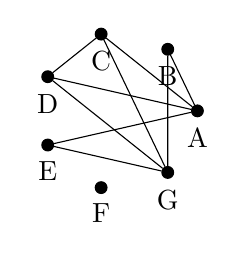
\begin{tikzpicture}[scale=1, every node/.style={draw,
            circle, fill=black, inner sep=1.5pt}]
            % Define nodes (vertices)
            \node(A) at (1,0) [label=below:A] {};
            \node(B) at ({cos(2*pi/7 r)}, {sin(2*pi/7 r)}) [label=below:B] {};
            \node(C) at ({cos(4*pi/7 r)}, {sin(4*pi/7 r)}) [label=below:C] {};
            \node(D) at ({cos(6*pi/7 r)}, {sin(6*pi/7 r)}) [label=below:D] {};
            \node(E) at ({cos(8*pi/7 r)}, {sin(8*pi/7 r)}) [label=below:E] {};
            \node(F) at ({cos(10*pi/7 r)}, {sin(10*pi/7 r)}) [label=below:F] {};
            \node(G) at ({cos(12*pi/7 r)}, {sin(12*pi/7 r)}) [label=below:G] {};

            \draw (A) -- (B);
            \draw (A) -- (C);
            \draw (A) -- (D);
            \draw (A) -- (E);
            \draw (G) -- (B);
            \draw (G) -- (C);
            \draw (G) -- (D);
            \draw (G) -- (E);
            \draw (C) -- (D);
          \end{tikzpicture}
        \end{center}
    \end{enumerate}
  \item We remove in the order $2, 3, 4, 1, 5$, yielding a Prufer
    list of $(6, 6, 1, 6, 6).$

  \item We decode using the standard algorithm, yielding:
    \begin{center}
      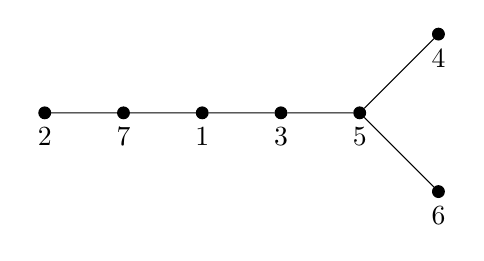
\begin{tikzpicture}[scale=1, every node/.style={draw, circle,
        fill=black, inner sep=1.5pt}]
        % Define nodes (vertices)
        \node(v2) at (0,0) [label=below:2] {};
        \node(v7) at (1,0) [label=below:7] {};
        \node(v1) at (2,0) [label=below:1] {};
        \node(v3) at (3,0) [label=below:3] {};
        \node(v5) at (4,0) [label=below:5] {};
        \node(v4) at (5,1) [label=below:4] {};
        \node(v6) at (5,-1) [label=below:6] {};

        \draw (v2) -- (v7) -- (v1) -- (v3) -- (v5) -- (v4);
        \draw (v5) -- (v6);
      \end{tikzpicture}
    \end{center}

\end{enumerate}
\end{document}
